\documentclass[twocolumn, 9pt]{extarticle}
\usepackage{amsmath}
\usepackage{lineno,hyperref}
\usepackage[table,x11names,dvipsnames,table]{xcolor}
\usepackage{authblk}
\usepackage{subcaption,booktabs}
\usepackage{graphicx}
\usepackage{multirow}
\usepackage[nolist,nohyperlinks]{acronym}
\usepackage[superscript]{cite}
\usepackage{tabularx}
\usepackage{float}
\usepackage[group-separator={,}]{siunitx}
\usepackage{geometry}
 \geometry{
 a4paper,
 papersize={210mm,279mm},
 left=12.73mm,
 top=20.3mm,
 marginpar=3.53mm,
 textheight=238.4mm,
 right=12.73mm,
 }


\setlength{\columnsep}{6.54mm}

%\linenumbers %%% Turn on line numbers here

\renewcommand{\familydefault}{\sfdefault}

\captionsetup[figure]{labelfont=bf,textfont=normalfont}
\captionsetup[subfigure]{labelfont=bf,textfont=normalfont}


%%%% comment out the below for the other title option
\makeatletter
\def\@maketitle{
\raggedright
\newpage
  \noindent
  \vspace{0cm}
  \let \footnote \thanks
    {\hskip -0.4em \huge \textbf{{\@title}} \par}
    \vskip 1.5em
    {\large
      \lineskip .5em
      \begin{tabular}[t]{l}
      \raggedright
        \@author
      \end{tabular}\par}
    \vskip 1em
  \par
  \vskip 1.5em
  }
\makeatother





\begin{document}


\title{Trip Duration Prediction Project Report}



\maketitle

\section{Introduction}

The NYC Taxi Duration Prediction competition on Kaggle challenges participants to build a model that predicts the total ride duration of taxi trips in New York City. The primary dataset is provided by the NYC Taxi and Limousine Commission and includes information such as pickup time, geo-coordinates, number of passengers, and other variables.

\section{Shape of the data}

\subsection{Target Variable (Trip Duration):}

The target variable distribution see Figure  \ref{fig:trip} looks like Gaussian distribution, there is a long right tail (right-skewed) which means that there are a few very long trips that may be outliers compared to the majority of trips.

\hfill \break
The peak of the distribution is around 5: This means that most trips are between 150 seconds and 1000 seconds (about 2.5 and 16.7 minutes) long

\hfill \break
The max trip duration took around 58771 minutes is approximately 40 days and 1111 minutes so definitely an outlier.

\hfill \break
Note: we perform  \[ \log(1 + x) \] transformation to Visualise better and \textbf{to help us with modeling large values.}


\begin{figure}[ht]
\centering
    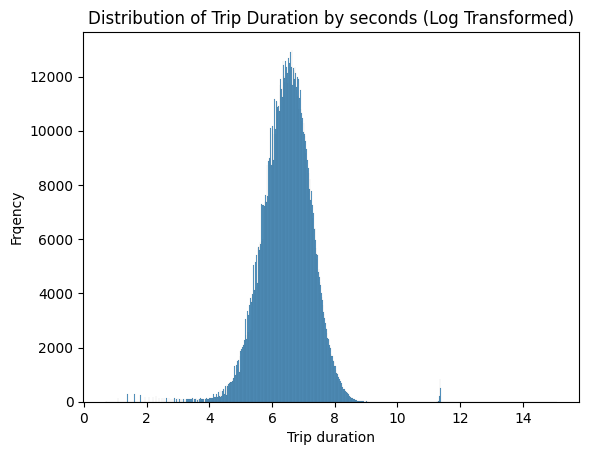
\includegraphics[width=\linewidth]{trip duration distriburion.png}
    \caption{\label{fig:trip}Trip duration distribution}
\end{figure}

\hfill \break
\subsection{Discrete Numerical Feature}

Vendor ID and passenger count are our Discrete Numerical Features.

\begin{figure}[ht]
\centering
    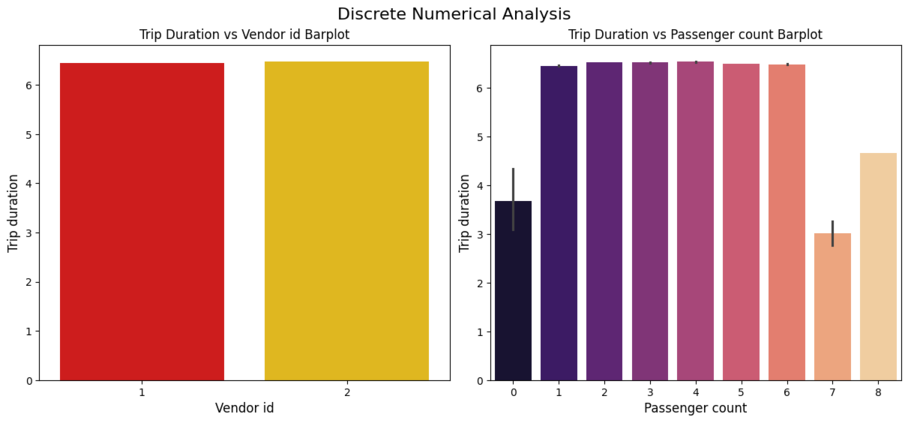
\includegraphics[width=0.55\textwidth, height=0.25\textheight]{Discrete Numerical Analysis.png}
    \caption{\label{Dis}Discrete Numerical Analysis}
\end{figure}

\hfill \break
Trip duration and Vendor ID: It's difficult to discern any clear patterns or trends between trip duration and vendor ID from the bar chart. The bars appear to be spread out relatively evenly across the x-axis, suggesting no significant difference in trip duration among vendors.

\hfill \break
When the number of passenger groups from [1 to 6] take constant trip duration and the number of passenger groups from [7 to 8] take less trip duration, Possible explanations:

\hfill \break
Vehicle Capacity: The vehicles used by both vendors may have a maximum capacity of 6 passengers. When there are 6 or fewer passengers, the vehicles are operating at their maximum capacity, and the trip duration remains constant because the vehicles are fully utilized.

\hfill \break
 Vehicle Type: It's also possible that the two vehicle vendors have different types of vehicles in their fleets. One vendor might have larger vehicles capable of accommodating more passengers, while the other vendor might have smaller vehicles. The larger vehicles can comfortably accommodate 7 to 8 passengers, resulting in shorter trip durations.
 
\hfill \break
Trip purpose: Trips with 7-8 passengers might be more likely to be for specific purposes (e.g., airport shuttle, group sightseeing) that involve shorter distances or routes optimised for efficiency.

\hfill \break
\textbf{ If vendor of the taxi not effect with trip duration so idea of vehicle type and vehicle capacity not correct so we need to use a boxplot  to detect If we just dealing with some random noise or passengers groups from [7 to 8] just travel less than another groups. }


\begin{figure}[ht]
\centering
    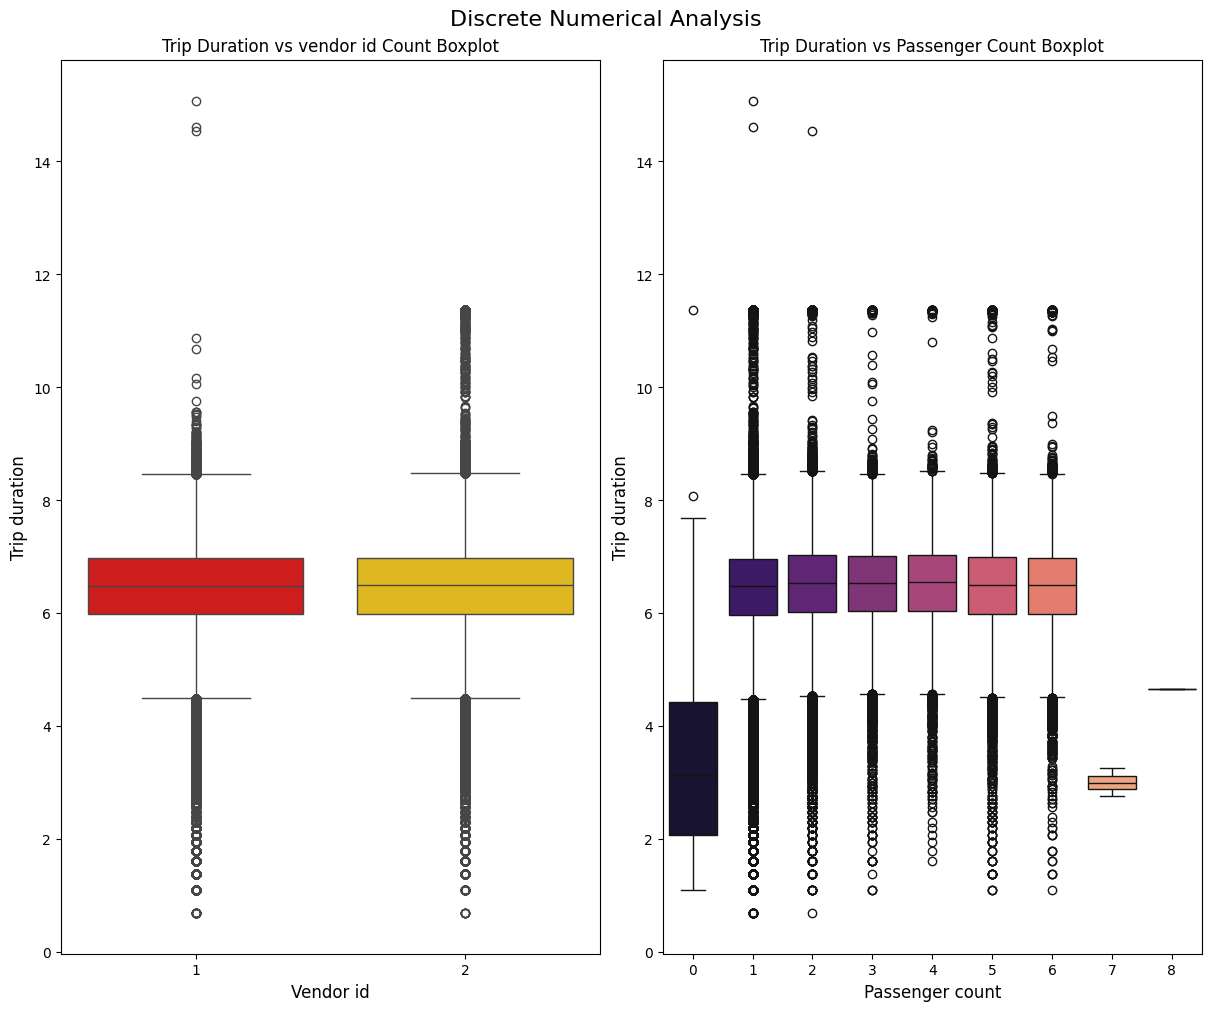
\includegraphics[width=0.50\textwidth, height=0.50\textheight]{boxplot.png}
    \caption{\label{fig:trip}Discrete Numerical Analysis (Boxplot)}
\end{figure}


\hfill \break
Trip duration distribution: The distribution of trip durations appears to be positively skewed for both groups, meaning there are more shorter trips than longer trips. This is especially evident for the group with lower passenger counts (left boxplot).


\hfill \break
Median trip duration: The median trip duration, represented by the horizontal line within the box, is longer for the group with higher passenger counts (right boxplot). This suggests that trips with more passengers tend to take longer overall.

\hfill \break
\textbf{Outliers:} There are a few outliers for both groups, represented by the circles beyond the whiskers. These are individual trips that were much longer than the majority of trips in their respective groups and this \textbf{Supports conclusion passengers groups from [7 to 8] just travel less than another groups because Trip purpose.}

\newpage
\subsection{Geographical Feature}

Using pickup latitude, pickup longitude, dropoff latitude and dropoff longitude we can calculate \href{https://en.wikipedia.org/wiki/Haversine_formula}{\textbf{haversine distance}}

\begin{figure}[ht]
\centering
    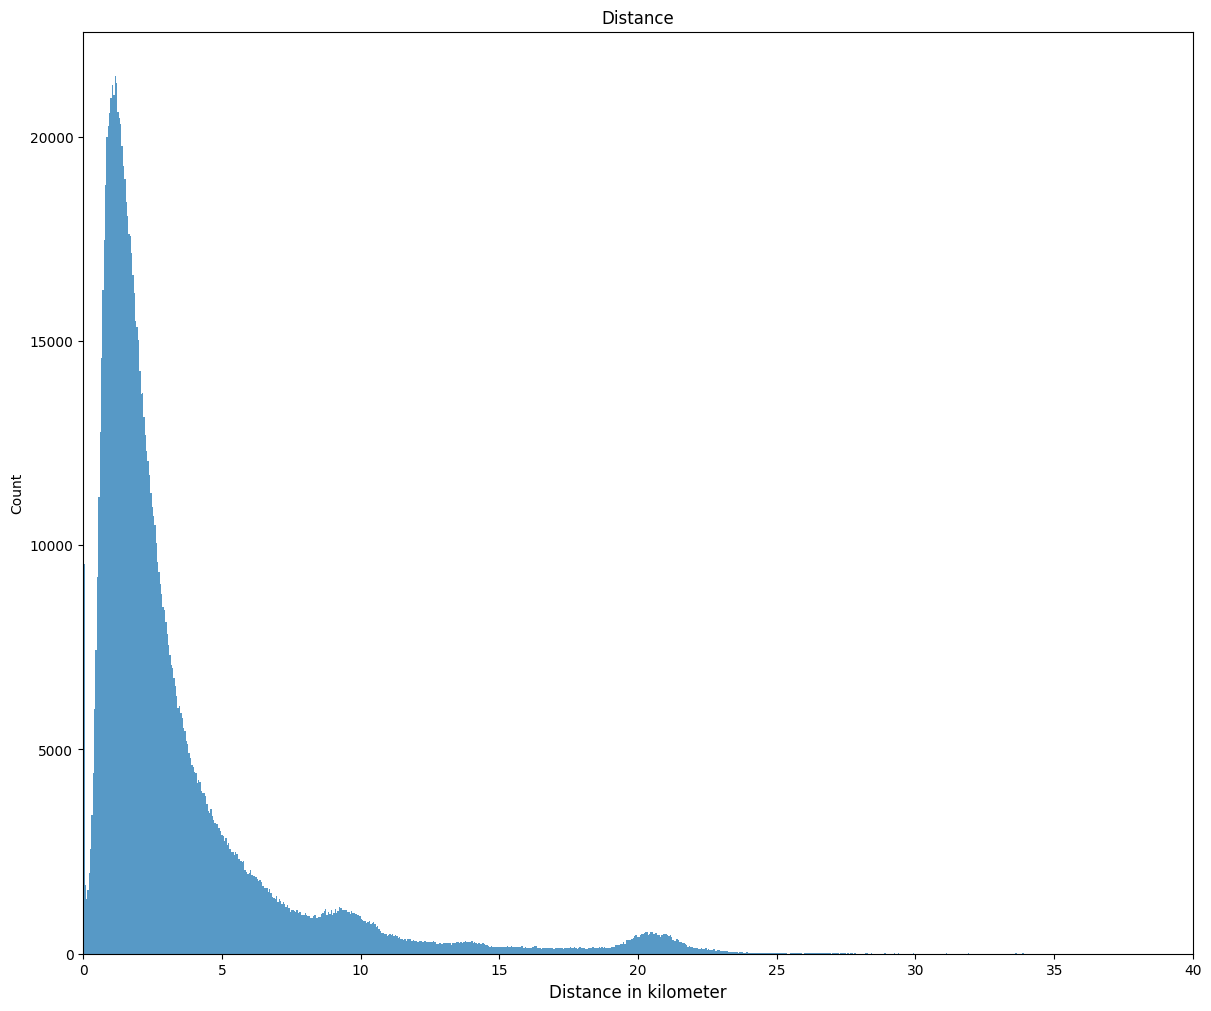
\includegraphics[width=0.55\textwidth, height=0.3\textheight]{haversine distance.png}
    \caption{\label{fig:distance}Haversine distance}
\end{figure}

\hfill \break
This distribution's right skewed So we can use a transformation
\[
\begin{aligned}
y' &= \log(x) \\
   &\text{or} \\
y' &= \sqrt{y}
\end{aligned}
\]
\textbf{which can improve the performance of our Linear model}

\hfill \break
Looks like most of the trip goes from less than 1 kilometre to 25 kilometres. Also, we have the trip duration and distance so we can calculate the speed of the trip

\begin{figure}[ht]
\centering
    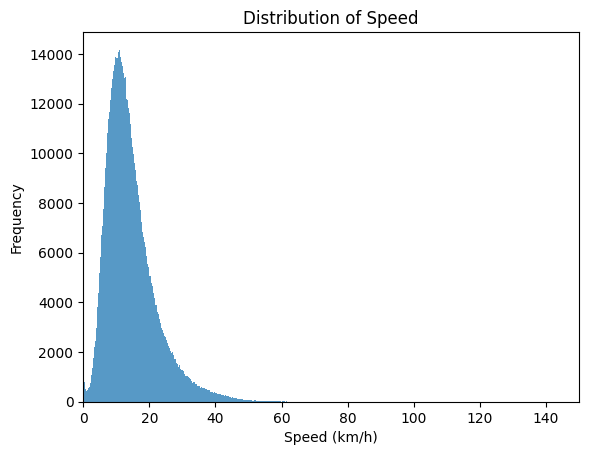
\includegraphics[width=0.5\textwidth, height=0.25\textheight]{Speed.png}
    \caption{\label{fig:speed} Distribution speed of the trips}
\end{figure}

\newpage
\subsection{Temporal/Time-date Analysis}

\hfill \break
Using data/time we can get new information like Months-day-Morning or afternoon or night-season for each trip and now we can try to find how it affects trip duration.

\begin{figure}[ht]
\centering
    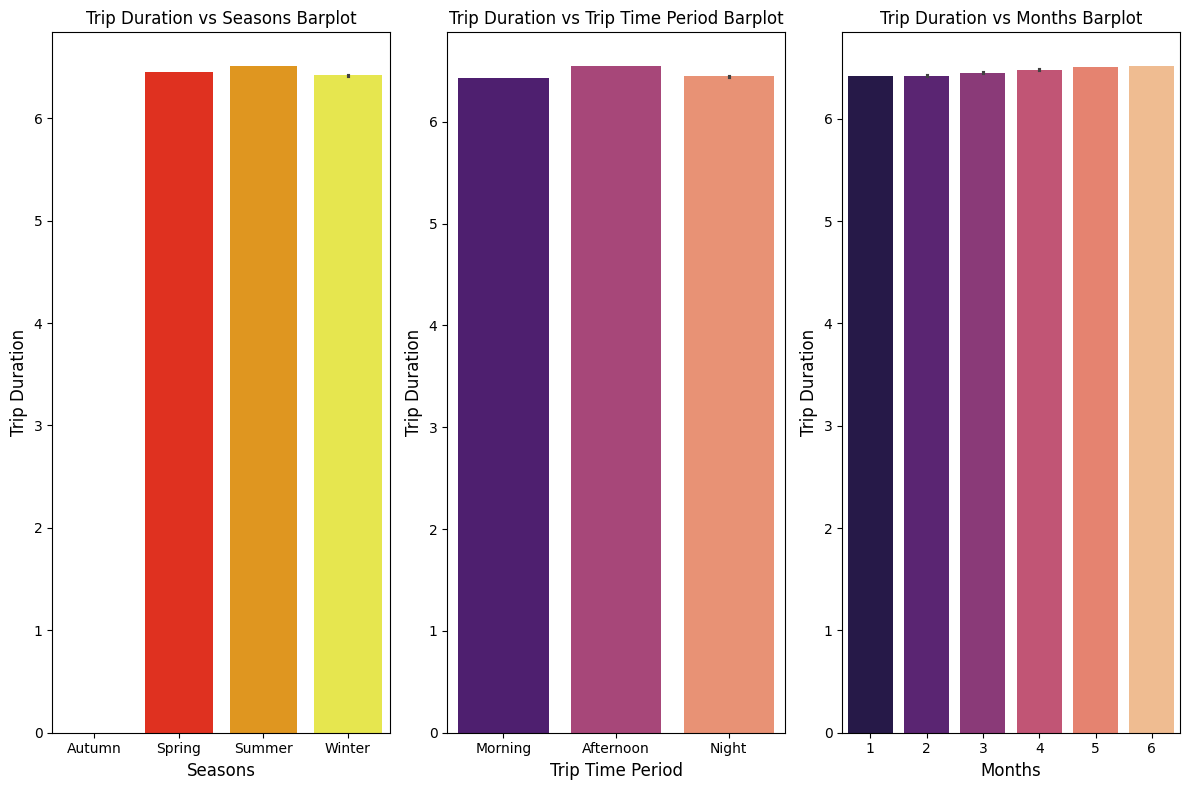
\includegraphics[width=0.4\textwidth, height=0.5\textheight]{time.png}
    \caption{\label{fig:time} Time-date Analysis}
\end{figure}


\hfill \break
The longer trip durations during summer might be attributed to vacations and holidays \ref{fig:time}, which lead to increased traffic on the roads.
Longer trip durations in the afternoon can be explained by higher levels of crowding during that time of day.
April, May, and July experience longer trip durations compared to other months.

\begin{figure}[ht]
\centering
    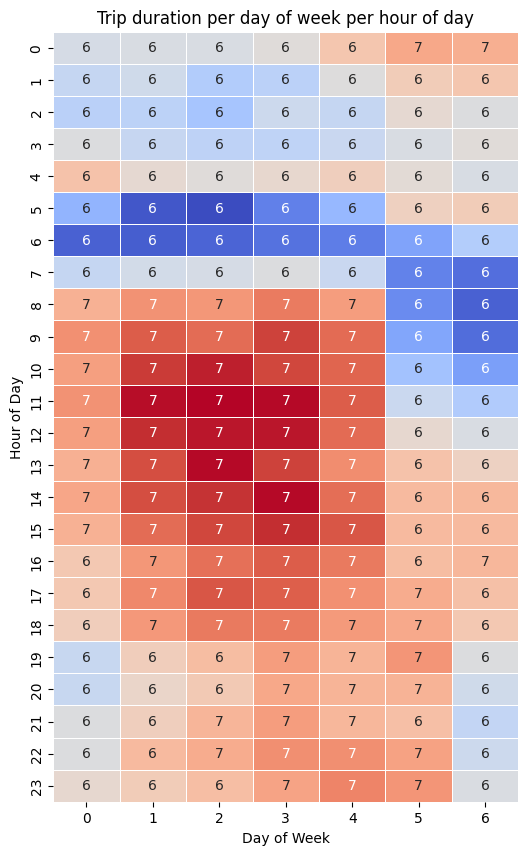
\includegraphics[width=0.4\textwidth, height=0.5\textheight]{weeks.png}
    \caption{\label{fig:time2} Time-date Analysis}
\end{figure}

\hfill \break
Trip durations are generally longer on weekends than on weekdays (Saturday and Sunday) \ref{fig:time2}.This is likely due to the fact that people are more likely to take longer trips for purposes on weekends.

\hfill \break
Trip durations are generally shorter during the morning and evening rush hours. This is likely due to the fact that people are more likely to be making shorter trips for commuting purposes during these times.

\hfill \break
Trip durations are generally longer in the middle of the day.This is likely due to the fact that people are more likely to be making longer trips for shopping, errands, or other activities during these times.


\newpage
\section{Correlation Analysis}

\hfill \break
Their positive relation trip duration (in Seconds log-Transformed) with pickup longitude, dropoff longitude and passenger count. Figure \ref{fig:crr}

\hfill \break
There negative relation trip duration (in Seconds log-Transformed) with pickup latitude and dropoff latitude. Figure \ref{fig:crr}

\hfill \break
\textbf{Their strong positive relation trip duration (in Seconds log-Transformed) with distance}. Figure \ref{fig:crr2}

\hfill \break
Their negative relation trip duration (in Seconds log-Transformed) with speed km/h. Figure \ref{fig:crr2}

\hfill \break
\textbf{Conclusion we have a pretty good relationship between the distance features and trip duration so we can use it in modeling}. Figure \ref{fig:crr2}


\begin{figure}[ht]
\centering
    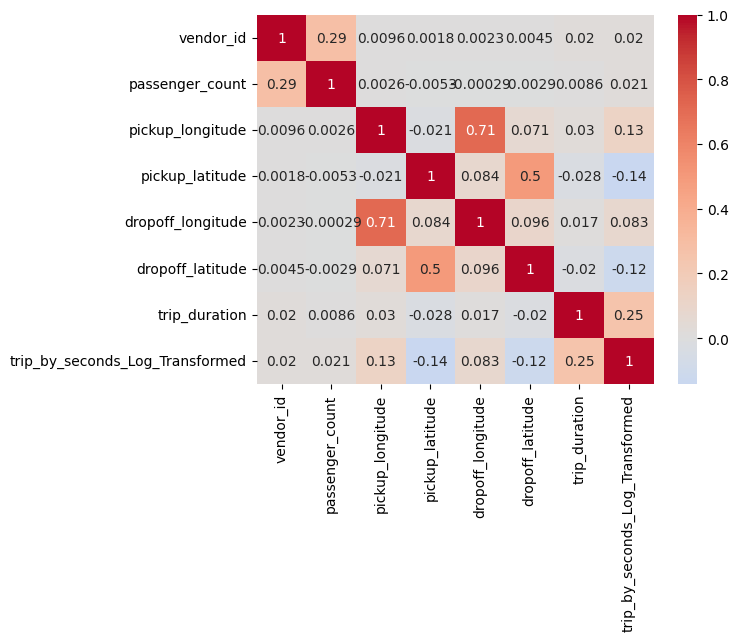
\includegraphics[width=1\linewidth]{crr.png}
    \caption{\label{fig:crr} Correlation Analysis}
\end{figure}

\hfill \break
\begin{figure}[ht]
\centering
    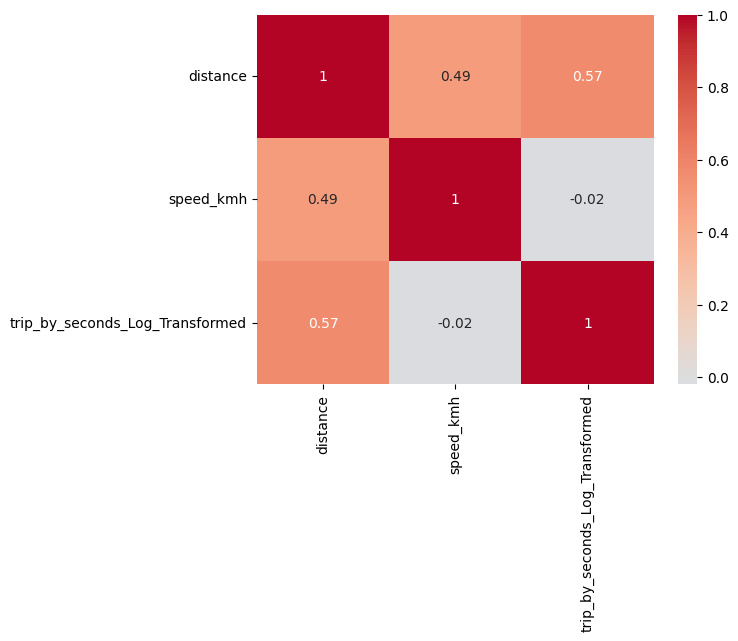
\includegraphics[width=1\linewidth]{crr2.png}
    \caption{\label{fig:crr2} Correlation Analysis}
\end{figure}

\begin{figure}
    \centering
    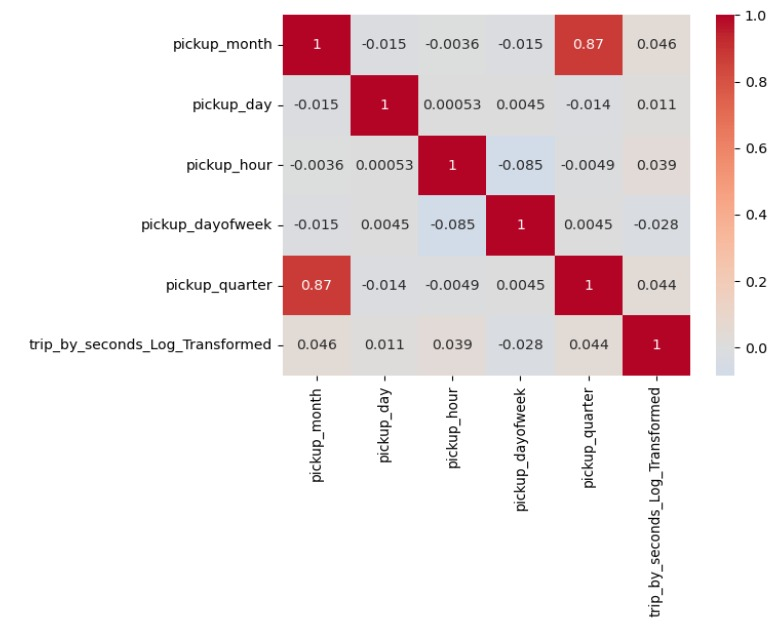
\includegraphics[width=1\linewidth]{corr3.png}
    \caption{Correlation Analysis}
    \label{fig:crr3}
\end{figure}


\newpage
\section{Modeling}
\hfill \break
The data pipeline splits the feature into categorical and numerical features.

\hfill \break
We perform One hot encoding for the categorical feature and For the numerical feature We scale the data by standard scalar then do Polynomial Features (degree=6) finally We use log transformation for the data.\textbf{ As previously discussed We perform log transformation because the distance data is right skewed.}

\subsection{Results}

\begin{table}[h]
\centering
\begin{tabular}{lcc}
\toprule
\textbf{Metric} & \textbf{Train} & \textbf{Validation} \\
\midrule
RMSE & 0.4376 & 0.4427 \\
R² & 0.6968 & 0.6938 \\
\bottomrule
\end{tabular}
\caption{Performance metrics for the model}
\label{tab:performance}
\end{table}


\subsection{Lessons and future work}

\hfill \break
Having a type of version control for the data or model scores is very beneficial for error analysis and verifying assumptions. In this project, we observed the following insights:

\begin{itemize}
    \item Feature selection consistently improves model performance.
    \item Outlier removal for intra-trip duration does not improve model performance.
\end{itemize}

\hfill \break
Building a separate pipeline to estimate the speed feature and using it as an input for predicting trip duration did not significantly improve the model's performance.

\hfill \break
Linear models often exhibit high bias. Given the characteristics of this dataset, it is important to explore more complex algorithms. For heterogeneous tabular data, techniques such as XGBoost and ensemble methods can be particularly effective.


\newpage
\begin{figure}
    \centering
    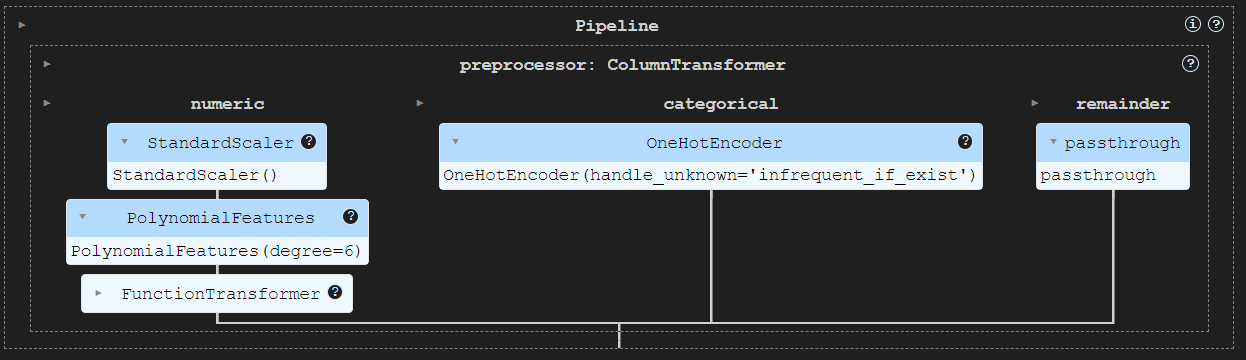
\includegraphics[width=1\linewidth]{Data Pipline.png}
    \caption{Data pipeline}
    \label{fig:Data pipeline}
\end{figure}



\end{document}